\documentclass[11pt,a4paper]{article}

\usepackage[utf8]{inputenc}
\usepackage[T1]{fontenc}
\usepackage{lmodern}
\usepackage[margin=0.95in]{geometry}
\usepackage{amsmath,amssymb}
\usepackage{booktabs}
\usepackage{graphicx}
\usepackage{xurl}
\usepackage{hyperref}
\usepackage{xcolor}
\usepackage{microtype}
\usepackage{enumitem}

\hypersetup{
  colorlinks=true,
  linkcolor=blue!60!black,
  citecolor=blue!60!black,
  urlcolor=teal!70!black,
  pdftitle={CRISOL-MBA-x64: Certified Neuro-Symbolic Deobfuscation of x86-64 Machine-Code Slices via Hybrid CEGIS and Lean 4 bv\_decide},
  pdfauthor={Luis Alejandro Arancibia}
}

\title{\textbf{CRISOL-MBA-x64: Certified Neuro-Symbolic Deobfuscation of x86-64 Machine-Code Slices via Hybrid CEGIS and Lean 4 \texttt{bv\_decide}}}

\author{
  Luis Alejandro Arancibia\\
  \textit{Computer Engineer (FIUBA, University of Buenos Aires)}\\
  \textit{Independent Researcher}\\
  ORCID: \href{https://orcid.org/0009-0003-6453-575X}{0009-0003-6453-575X}\\
  \texttt{arancibialuisalejandro@gmail.com}
}

\date{November 2026}

\begin{document}
\maketitle

\begin{abstract}
Mixed Boolean-Arithmetic (MBA) obfuscation remains a primary barrier in binary reverse engineering, malware analysis, and security auditing. Algebraic simplifiers such as SiMBA, GAMBA, ProMBA, and RUMBA achieve high speed on pure expression trees, yet fail when obfuscation is compiled into real x86-64 machine code entangled with carry-flag propagation (\texttt{ADC}/\texttt{SBB}), 32-to-64-bit zero-extension, arithmetic shifts (\texttt{SAR}), and bit rotations (\texttt{ROL}/\texttt{ROR}). Conversely, neural approaches such as LLM4Decompile and gMBA operate on string expressions or evaluate only finite test-case re-executability without universal formal guarantees, exposing analysts to silent edge-case hallucinations.

We present \textbf{CRISOL-MBA-x64}, a certified neuro-symbolic deobfuscation framework that pairs LLM candidate synthesis with a zero-LLM-trust verification pipeline that is sound relative to the declared Trusted Computing Base (TCB): a minimalist x86-64 lifter empirically cross-checked on 1,024 concrete vectors per test (0 discrepancies across 82,944 three-way checks: 31,744 direct CPU-vs.-Unicorn-vs.-lifter instruction checks plus 51,200 CPU-vs.-Unicorn-vs.-reference-expression slice checks across 28 sanity and 22 $V_{\mathrm{real}}$ slices), a vectorized concrete pre-filter, dual \texttt{QF\_BV} SMT solvers (Bitwuzla + Z3), and independently checked \textbf{LRAT} SAT proof certificates (\texttt{CaDiCaL} + \texttt{lrat-check}) as well as \textbf{Lean 4 \texttt{bv\_decide}} proof certificates that verify bit-blasting inside Lean.

Following our study protocol with disjoint identity templates (disclosing freeze- and baseline-scope deviations in Section~4), we evaluate CRISOL-MBA-x64 across three frozen benchmarks:
(1)~\textbf{Benchmark 1 ($V_{\mathrm{test}}$, $N=160$ straight-line x86-64 slices across 8 algebraic templates $\times 20$ immediate-constant variants, 60\,s budget):} under a \textbf{strict $\le 60.0$\,s wall-clock cutoff} (and in-flight completion in parentheses), the best non-LLM baseline (\texttt{SiMBA} + cost-bounded enumerator + Xyntia/STOKE-style MCMC-CEGIS, $A \cup C$) certifies \textbf{24.38\%: 39/160} (in-flight: 26.25\%, 42/160), while official Denuvo \textbf{GAMBA} emits \texttt{simplified} output (unverified for LRAT/cost; 120 slices filtered out prior to invocation by our single-AST adapter) on \textbf{40/40 (100\%)} of the two pure-algebraic 64-bit families (40/160 = 25.00\% overall). CEGIS configuration $D$ reaches \textbf{90.62\%: 145/160} (in-flight: 91.25\%, 146/160; $+66.25$\,pp strict vs.\ $A \cup C$, instance-level exact McNemar $p = 2.47 \times 10^{-32}$; family-level sign test: 7 wins, 1 tie, 0 losses, two-sided $p = 0.0156$; and \textbf{121/129 vs.\ 32/129}, $+68.99$\,pp on the $\le 10$\,s post-prefilter freeze subset), whereas pre-registered $H_2$ ($D > B$) is \textbf{not confirmed} ($B$ reaches \textbf{96.25\%: 154/160}). Exploratory (post-hoc) Hybrid $H$ ($K=6 \to$ CEGIS fallback) achieves \textbf{99.38\%: 159/160 under strict $\le 60.0$\,s} (95\% Clopper-Pearson CI $[96.6\%, 100\%]$; $+75.00$\,pp vs.\ $A \cup C$, $p = 1.50 \times 10^{-36}$) and \textbf{100.0\%: 160/160} in-flight (one slice at \textbf{74.29\,s}) with \texttt{gemini-4-hydrogen} (Medium)---and \textbf{119/120 (99.17\%) strict} vs.\ $19/120$ ($15.83\%$) excluding both \texttt{nand\_nor\_add\_64} and \texttt{sar\_neg\_32}---plus \textbf{100.0\%: 40/40} ($\max 38.71$\,s) with \texttt{gpt-6.2-sol}.
(2)~\textbf{Benchmark 2 ($V_{\mathrm{hard}}$, $N=40$ \texttt{IMUL} ground-truth equivalence proofs $F_B \equiv g$, re-run under equalized 30.0\,s solver caps):} under a \textbf{strict $\le 30.0$\,s recorded solver/certifier cutoff}, uncertified Bitwuzla closes 40/40, Z3 \texttt{QF\_BV} closes \textbf{0/40 (0.0\%)}, and raw Z3 bit-blasting + CaDiCaL LRAT closes \textbf{2/40 (5.0\%)} (3/40 = 7.5\% in-flight at 33.29\,s); \textbf{Lean 4 \texttt{bv\_decide}} raises certified proofs to \textbf{87.5\% (35/40, all $\le 30.0$\,s)}: \textbf{20/20 (100\%)} on 32-bit \texttt{IMUL} (5.41\,s mean) and \textbf{15/20 (75\%)} on 64-bit \texttt{IMUL} (10.57\,s 64-bit mean; 7.99\,s overall mean across all 40 slices).
(3)~\textbf{Benchmark 3 ($V_{\mathrm{real}}$, $N=22$ \texttt{-O2 -fno-inline} binaries across 4 C templates: 10 \texttt{affine\_mul\_64}, 10 \texttt{hash\_mix\_64}, 1 \texttt{4var\_token\_64}, 1 \texttt{signed\_shift\_32}):} non-LLM baselines $A$ and $C$ solve \textbf{0/22 (0.0\%)}, whereas \textbf{Hybrid $H$ + Lean 4 \texttt{bv\_decide}} certifies \textbf{22/22 (100.0\%; $\max 31.64$\,s; 95\% CI $[84.6\%, 100\%]$; $p = 4.77 \times 10^{-7}$)} in 23.44\,s mean time (\texttt{H-sol}: 6/22 = 27.27\%, $p = 0.031$, not significant at $\alpha = 0.01$).
Mutation testing and pre-filter-evading negatives yielded 0 false positives, and all 362 Phase~1 \texttt{PASS} entries record verified \texttt{lrat\_sha256} digests.
\end{abstract}

\section{Introduction}

Software protection schemes, digital rights management (DRM), and malware routinely apply Mixed Boolean-Arithmetic (MBA) obfuscation to replace simple arithmetic or bitwise operations with mathematically equivalent yet structurally opaque combinations of $+$, $-$, $*$, $\&$, $|$, $\oplus$, and $\sim$~\cite{mbablast2021,simba2022}. When lowered by optimizing compilers (\texttt{gcc -O2}, \texttt{clang -O2}) or assembly-level obfuscators into x86-64 machine code, basic blocks entangle MBA identities with architecture-specific semantics: explicit Carry Flag (\texttt{CF}) chains via \texttt{ADC}/\texttt{SBB}, implicit zero-extension of 32-bit register writes into 64-bit registers, arithmetic right shifts (\texttt{SAR}), and bit rotations (\texttt{ROL}/\texttt{ROR}).

Existing deobfuscation paradigms face a three-way impasse:
\begin{itemize}[leftmargin=1.5em]
  \item \textbf{Algebraic MBA solvers} (MBA-Blast~\cite{mbablast2021}, SiMBA~\cite{simba2022}, GAMBA~\cite{gamba2023}, ProMBA~\cite{promba2023,promba2026tosem}, RUMBA~\cite{rumba2026}) operate on pure expression ASTs over $\mathbb{Z}_{2^n}$ without modeling x86-64 carry flags, rotations, or 32-to-64-bit zero-extension directly.
  \item \textbf{Black-box search and superoptimization} (STOKE~\cite{stoke2013}, Xyntia~\cite{xyntia2021}) handle arbitrary machine semantics via I/O traces, but suffer combinatorial explosion once expressions combine 3--4 inputs, carry flags, shifts, and rotations.
  \item \textbf{Neural decompilation and MBA translation} (LLM4Decompile~\cite{llm4decompile2024}, gMBA~\cite{gmba2025}) recover readable approximations, yet operate on expression strings without binary semantics (gMBA) or evaluate only finite test-case re-executability (LLM4Decompile), offering zero guarantee against edge-case divergence on $2^{64}$ bit-vector inputs.
\end{itemize}

\textbf{Key insight.} In formal mathematics, LLMs achieve breakthroughs when paired with a \emph{deterministic verification oracle}: finding a candidate proof or simplified form is hard, but checking universal equivalence is objective and machine-verifiable. \textbf{CRISOL-MBA-x64} transfers this principle to straight-line x86-64 binary deobfuscation, separating untrusted candidate synthesis from certified formal verification backed by SMT solvers~\cite{z3_2008,bitwuzla2023}, LRAT SAT proofs~\cite{lrat2017,cadical2024}, and Lean~4~\cite{lean4_2021}.

\section{Related Work}

Table~\ref{tab:related} situates CRISOL-MBA-x64 against prior algebraic, search-based, and neural deobfuscation systems.

\begin{table}[htbp]
\centering
\scriptsize
\resizebox{\textwidth}{!}{%
\begin{tabular}{@{}llllll@{}}
\toprule
\textbf{System} & \textbf{Venue / Year} & \textbf{Domain} & \textbf{Neural Prior} & \textbf{x86-64 (\texttt{CF}, 32$\to$64)} & \textbf{Checkable Cert.} \\
\midrule
STOKE~\cite{stoke2013} & ASPLOS '13 & x86-64 superopt & No (MCMC) & Yes & No (SMT trusted) \\
MBA-Blast~\cite{mbablast2021} & USENIX Sec '21 & Linear MBA AST & No & No & No \\
Xyntia~\cite{xyntia2021} & ACM CCS '21 & Black-box slices & No (Local) & Yes (I/O trace) & No (probabilistic) \\
SiMBA~\cite{simba2022} & CheckMATE '22 & Linear MBA AST & No & No & No \\
GAMBA~\cite{gamba2023} & EuroS\&PW '23 & General MBA AST & No & No & Optional Z3 \\
ProMBA~\cite{promba2023,promba2026tosem} & CCS '23 / TOSEM '26 & MBA AST & No (Synth+E-sat) & No & No \\
LLM4Decompile~\cite{llm4decompile2024} & EMNLP '24 & Asm $\to$ C & Yes & Partial (tests) & No \\
gMBA~\cite{gmba2025} & ACL Findings '25 & MBA strings & Yes (Transformer) & No & No \\
RUMBA~\cite{rumba2026} & HAL '26 & Linear/Poly MBA & No & No & No \\
\textbf{CRISOL-MBA-x64} & \textbf{2026} & \textbf{x86-64 bytes} & \textbf{Yes (Hybrid CEGIS)} & \textbf{Yes (Native-checked)} & \textbf{LRAT + Lean 4 \texttt{bv\_decide}} \\
\bottomrule
\end{tabular}%
}
\caption{Comparison with state-of-the-art algebraic, search-based, and neural MBA deobfuscators.}
\label{tab:related}
\end{table}

\section{Formal Problem Statement and Trusted Computing Base}

Let $B \in \{0,1\}^{8L}$ be a straight-line, register-only x86-64 byte sequence of at most 24 instructions drawn from a closed allowlist of 17 mnemonics:
\begin{align*}
\mathcal{M} = \{\,&\texttt{MOV}, \texttt{LEA}_{\mathrm{reg}}, \texttt{ADD}, \texttt{ADC}, \texttt{SUB}, \texttt{SBB}, \texttt{NEG}, \texttt{IMUL}_{\mathrm{non\text{-}nested}},\\
&\texttt{AND}, \texttt{OR}, \texttt{XOR}, \texttt{NOT}, \texttt{SHL}/\texttt{SAL}, \texttt{SHR}, \texttt{SAR}, \texttt{ROL}, \texttt{ROR}\,\}
\end{align*}
with immediate shift/rotate counts and no memory accesses, stack-pointer (\texttt{rsp}) operands, branches, or system calls. Under our execution contract (rejecting \texttt{rsp}/\texttt{esp}/\texttt{sp}/\texttt{spl} at decode time, initializing the 11 non-input GPRs \texttt{rax}, \texttt{rbx}, \texttt{rbp}, \texttt{r8}--\texttt{r15} to $0$ in both the native/Unicorn harness and the lifter, and truncating/zero-extending 32-bit \texttt{0x67} address-size \texttt{LEA} effective addresses per Intel SDM Table~3-54), $B$ defines a deterministic bit-vector function $F_B : (\mathrm{BV}_{64})^4 \times \mathrm{BV}_1 \to \mathrm{BV}_{64}$, mapping $(\texttt{rdi}, \texttt{rsi}, \texttt{rdx}, \texttt{rcx}, \texttt{cf}) \mapsto \texttt{rax}_{\mathrm{out}}$. Given a canonical functional bit-vector grammar $\mathcal{G}$, a CSE + constant-folding cost metric $\mathrm{Cost}(\cdot)$, ground-truth cost $c_g$, and margin $\varepsilon = 0.10$, a candidate $e \in \mathcal{G}$ is a \textbf{certified simplification} iff $\mathrm{Cost}(e) \le (1+\varepsilon)\,c_g$ and $\forall \vec{x},\ F_B(\vec{x}) = [\![ e ]\!](\vec{x})$ is backed by an independently verified certificate (LRAT via \texttt{lrat-check}~\cite{lrat2017} or a Lean~4 \texttt{bv\_decide} proof~\cite{lean4_2021}).

\paragraph{Explicit TCB Boundary.}
Our verification pipeline is sound \emph{relative to the declared TCB}:
\begin{itemize}[leftmargin=1.5em]
  \item Under \texttt{CaDiCaL}~\cite{cadical2024} + \texttt{lrat-check}~\cite{lrat2017}, the SAT solver is outside the TCB while Z3's bit-blaster~\cite{z3_2008} remains inside.
  \item Under \textbf{Lean 4.36.0 \texttt{bv\_decide}}~\cite{lean4_2021}, bit-blasting is formally verified inside Lean; running \texttt{\#print axioms} on our generated theorems reports \texttt{[propext, Classical.choice, Quot.sound, <thm>.\_native.bv\_decide.ax\_*]}, reflecting Lean~4.36.0's theorem-scoped native-evaluation axiom. Thus Lean's kernel, Lean's compiler/runtime (for native reflection), our Python theorem emitter (\texttt{oracle\_lean.py}), and the minimalist x86-64 lifter remain in the TCB.
  \item Lifter fidelity ($B \to F_B$) is empirically anchored—not formally mechanized—by our Sanity Gate (\textbf{82,944 three-way checks} at 1,024 concrete vectors per test, 0 discrepancies): 31 closed-list instruction unit tests (\textbf{31,744} direct native-CPU vs.\ Unicorn~\cite{unicorn2015} vs.\ \texttt{QF\_BV}-lifter checks) plus 28 dataset-sanity and 22 $V_{\mathrm{real}}$ slices (\textbf{51,200} native-CPU vs.\ Unicorn vs.\ ground-truth expression checks, linked to the lifter by SMT/Lean equivalence).
\end{itemize}

\section{System Architecture and Experimental Protocol}

CRISOL-MBA-x64 runs entirely on CPU (18 vCPU, 94\,GB RAM, Linux x86-64, no GPU) in five stages:
(0)~\texttt{capstone}~\cite{capstone2014} decodes bytes and enforces $\mathcal{M}$ and the 24-instruction cap at 0 tokens;
(1)~candidate synthesis via $A$ (exact SiMBA basis solver + cost-bounded enumerator), $C$ (Xyntia/STOKE-style MCMC-CEGIS without LLM), $B$ (LLM One-Shot, $K=8$), $D$ (Sequential CEGIS, $4\times 2$ with concrete counterexample feedback), or $H$ (Hybrid Wide One-Shot $K=6 \to$ CEGIS $2\times 2$ fallback);
(2)~\texttt{numpy} concrete pre-filter on 1,024+ boundary, one-hot, and counterexample vectors (rejects only, never approves);
(3)~dual \texttt{QF\_BV} miter in Bitwuzla~\cite{bitwuzla2023} and Z3~\cite{z3_2008} with native CPU replay of every \texttt{SAT} counterexample (non-reproducing \texttt{SAT} triggers \texttt{LIFTER\_BUG}, counted as \texttt{FAIL}; 0 final instance verdicts were \texttt{LIFTER\_BUG}); and
(4)~mandatory certificate checking via \texttt{CaDiCaL 3.1.0 --lrat=true --binary=false} + \texttt{lrat-check} (with deterministic DIMACS header normalization fixing Z3's \texttt{goal.dimacs()} off-by-one \texttt{max\_var} bug) or \textbf{Lean 4.36.0 \texttt{bv\_decide}}.

\paragraph{Models and CLI Invocation.}
All LLM experiments were executed on November~23, 2026 using two publicly available models via local CLI wrappers:
(a)~\texttt{gemini-4-hydrogen} (Medium reasoning variant, invoked via \texttt{agy 1.5.15} with \texttt{--model} \texttt{gemini-4-hydrogen-medium} \texttt{--disable-slash-commands -p}; single-turn text prompt with slash commands disabled, though without an explicit CLI tool-denial flag); and
(b)~\texttt{gpt-6.2-sol} (invoked via \texttt{codex-cli 0.170.0} with \texttt{codex exec -m gpt-6.2-sol} \texttt{-c model\_reasoning\_effort="low"} \texttt{--skip-git-repo-check} \texttt{--sandbox read-only}).
Regardless of how candidates are produced, every candidate is strictly parsed into $\mathcal{G}$ and independently verified from scratch by Stages~2--4.

\paragraph{Protocol Specification, Deviations, and Anti-Leakage.}
Hypotheses ($H_1$: $D$ exceeds $A \cup C$ by $\ge +15$\,pp; $H_2$: $D$ exceeds $B$; $\varepsilon = 0.10$, exact paired McNemar $\alpha = 0.01$), instruction allowlists, and Go/No-Go criteria were drafted locally prior to test execution in \texttt{docs/experimental-protocol.md} with SHA-256 dataset manifests (\texttt{data/manifest\_V.sha256}); because that document and the initial Phase~1 logs were pushed together in public commit \texttt{8008d30}, GitHub anchors content integrity rather than an external pre-execution timestamp. We disclose four implementation deviations relative to that protocol document:
(i)~during dataset freeze, \texttt{run\_experiment.py} admitted any LRAT-certified slice into $V_{\mathrm{test}}$ ($N=160$) rather than enforcing $\text{\texttt{gt\_cert\_sec}} \le 10.0$\,s (where \texttt{gt\_cert\_sec} starts after concrete pre-filter initialization: 129/160 satisfied $\le 10.0$\,s, while 31 took 10.0--16.45\,s; we report $H_1$ on both $N=160$ and $N=129$, and did not re-run the 1,024-vector CPU-vs.-Unicorn check on every generated test slice beyond the 28 sanity and 22 $V_{\mathrm{real}}$ slices);
(ii)~\texttt{generator.py} instantiated 20 randomized immediate-constant variants per family from 8 disjoint algebraic templates (fixing register operands per template) and deduplicated exact byte sequences rather than normalizing modulo constants, so instance-level McNemar tests treat template variants as observations (we therefore pair them with a family-level sign test);
(iii)~baseline $A$ implemented linear SiMBA + cost-bounded enumeration without degree-2 polynomial interpolation or Z3 simplification, and both $A$ and $C$'s search grammars omitted \texttt{ashr} (affecting \texttt{sar\_neg\_32}); and
(iv)~the LLM prompt's grammar formatting example (\texttt{xor(add(rdi, rsi), 0x1234)}) matches the outer structure of \texttt{nand\_nor\_add\_64} (where $A \cup C$ already scores 20/20; we therefore report a joint $N=120$ sensitivity analysis excluding both \texttt{nand\_nor\_add\_64} and \texttt{sar\_neg\_32}).
Four development templates ($V_{\mathrm{dev}}=40$) remained strictly disjoint from ten test templates ($V_{\mathrm{test}}=160$, $V_{\mathrm{hard}}=40$).

\section{Evaluation Results}

\subsection{Benchmark 1: Blind Out-of-Sample Evaluation on $V_{\mathrm{test}}$ ($N=160$)}

Because our runner checks the 60\,s budget before launching each synthesis/verification step (allowing an already-started in-flight step to complete rather than killing subprocesses mid-flight), Table~\ref{tab:vtest} and Figure~\ref{fig:vtest} report \textbf{both} the strict post-hoc $\le 60.0$\,s wall-clock cutoff and the in-flight loop-gate completion counts.

\begin{table}[htbp]
\centering
\footnotesize
\resizebox{\textwidth}{!}{%
\begin{tabular}{@{}llrrrrrr@{}}
\toprule
\textbf{Config} & \textbf{Description} & \textbf{Strict $\le 60$\,s} & \textbf{Strict (\%)} & \textbf{In-Flight} & \textbf{In-Flight (\%)} & \textbf{Mean / Max (s)} & \textbf{LLM Calls} \\
\midrule
$A$ & SiMBA + cost-bounded enumerator (LRAT) & 20 / 160 & 12.50 & 20 / 160 & 12.50 & 0.88 / 3.27 & 0.00 \\
GAMBA & Official Denuvo GAMBA (\texttt{simplified} on 2 AST fams, \emph{unverif.}) & 40 / 160 & 25.00 & 40 / 160 & 25.00 & --- & 0.00 \\
$C$ & Xyntia/STOKE MCMC-CEGIS (No-LLM, LRAT) & 39 / 160 & 24.38 & 42 / 160 & 26.25 & 50.50 / 65.75 & 0.00 \\
$A \cup C$ & Virtual best non-LLM baseline (certified) & 39 / 160 & 24.38 & 42 / 160 & 26.25 & --- & 0.00 \\
$A \cup C \cup \text{GAMBA}$ & Union incl.\ GAMBA \texttt{simplified} (\emph{unverif.}) & 55 / 160 & 34.38 & 56 / 160 & 35.00 & --- & 0.00 \\
$B$ & LLM One-Shot (\texttt{gemini-4-hydrogen}, $K=8$) & 154 / 160 & 96.25 & 154 / 160 & 96.25 & 25.29 / 68.30* & 1.00 \\
$D$ & \textbf{Pre-reg.\ CEGIS} ($4\times 2$, LRAT) & \textbf{145 / 160} & \textbf{90.62} & \textbf{146 / 160} & \textbf{91.25} & 26.65 / 63.96 & 1.32 \\
$H$ (Hydrogen) & \emph{Exploratory} Hybrid ($6 \to 2\times 2$, LRAT) & \textbf{159 / 160} & \textbf{99.38} & \textbf{160 / 160} & \textbf{100.00} & 29.60 / 74.29 & 1.01 \\
$H$ (GPT-6.2-Sol) & \emph{Exploratory} stratified cross-family ($N=40$) & \textbf{40 / 40} & \textbf{100.00} & \textbf{40 / 40} & \textbf{100.00} & 28.51 / 38.71 & 1.00 \\
\bottomrule
\end{tabular}%
}
\caption{Benchmark 1 ($V_{\mathrm{test}}$, $N=160$, 8 disjoint x86-64 templates; 0 final \texttt{LIFTER\_BUG} verdicts). *All 154 passes of $B$ completed in $\le 60.0$\,s (68.30\,s occurred on a failing slice).}
\label{tab:vtest}
\end{table}

\begin{figure}[htbp]
\centering
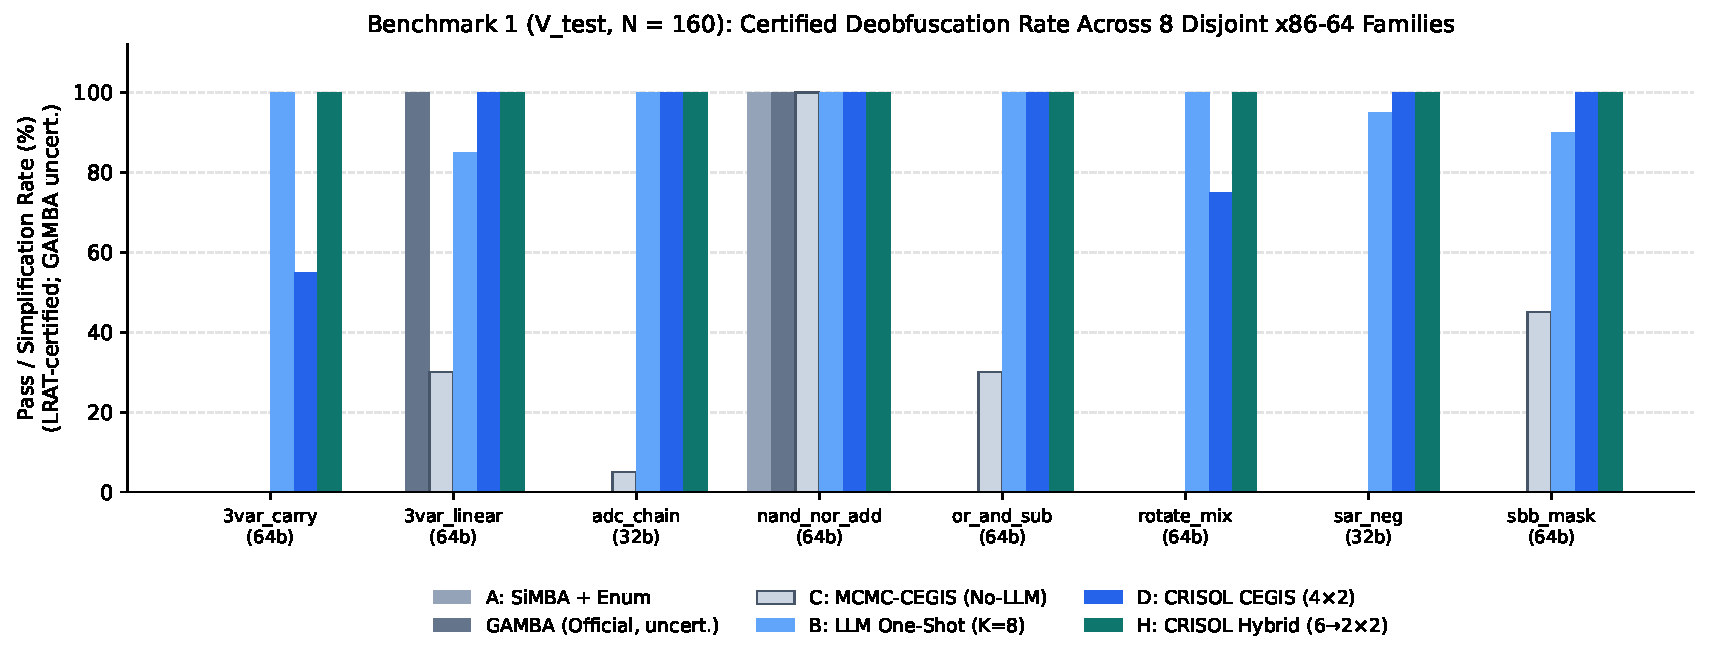
\includegraphics[width=\textwidth]{fig1_vtest_ablation.pdf}
\caption{Certified pass rates across the 8 disjoint x86-64 families of $V_{\mathrm{test}}$ ($N=160$, loop-entry 60\,s budget; under strict $\le 60.0$\,s, $C=39$, $D=145$, $H=159$).}
\label{fig:vtest}
\end{figure}

\begin{itemize}[leftmargin=1.5em]
  \item \textbf{Hypothesis $H_1$ ($D$ vs.\ $A \cup C$, $+15$\,pp threshold) and sensitivity checks:} Instance-level McNemar supports $H_1$ on $V_{\mathrm{test}}$ ($N=160$: strict $\le 60.0$\,s gives $+66.25$\,pp, $n_{10}=106, n_{01}=0, p = 2.47 \times 10^{-32}$; in-flight $+65.00$\,pp, $p = 9.86 \times 10^{-32}$) and on the $\text{\texttt{gt\_cert\_sec}} \le 10.0$\,s subset ($N=129$: $121/129 = 93.80\%$ vs.\ $32/129 = 24.81\%$, $+68.99$\,pp, $p = 3.23 \times 10^{-27}$). At the template level ($N=8$ families), $D$ beats $A \cup C$ on 7 families and ties on 1 (\texttt{nand\_nor\_add\_64}: 20/20 each; exact two-sided sign test $p = 0.0156$, one-sided $p = 0.0078$). Excluding \textbf{both} \texttt{nand\_nor\_add\_64} (prompt example structure) and \texttt{sar\_neg\_32} (missing \texttt{ashr} in $A$/$C$), on the remaining $N=120$ slices $D$ still beats $A \cup C$ by \textbf{105/120 (87.50\%) vs.\ 19/120 (15.83\%)} ($+71.67$\,pp, $p = 2.58 \times 10^{-26}$), and $H$ reaches \textbf{119/120 (99.17\%) strict} ($+83.33$\,pp, $p = 1.58 \times 10^{-30}$; 120/120 in-flight).
  \item \textbf{Hypothesis $H_2$ ($D$ vs.\ $B$):} \textbf{NOT CONFIRMED.} $D$ ($145/160$ strict; $146/160$ in-flight, sampling $K=2$ candidates per round for up to 4 rounds) trailed One-Shot $B$ ($154/160$, sampling $K=8$ in a single call; exact McNemar $n_{10}=6, n_{01}=15, p = 0.078$ strict; $n_{10}=6, n_{01}=14, p = 0.115$ in-flight). Of the 6 slices passed by $D$ but missed by $B$, 4 succeeded in Round~1 and 2 in Round~2 (each after a Round~1 call with 0 parseable candidates).
  \item \textbf{Exploratory Hybrid $H$:} Designed post-hoc after observing $B$ vs.\ $D$, $H$ achieves \textbf{159/160 (99.38\%, 95\% CI $[96.6\%, 100\%]$)} under strict $\le 60.0$\,s ($+75.00$\,pp vs.\ $A \cup C$, $p = 1.50 \times 10^{-36}$; vs.\ $B$, $n_{10}=6, n_{01}=1, p = 0.125$) and \textbf{160/160 (100.0\%, 95\% CI $[97.7\%, 100\%]$)} in-flight (one slice \texttt{3var\_carry\_64\_020} finished at \textbf{74.29\,s}) in 1.01 mean LLM calls.
  \item \textbf{GAMBA scope and wrapper boundary:} Official GAMBA returned non-error \texttt{simplified} expressions on \textbf{40/40 (100\%)} of the two pure-algebraic 64-bit families (\texttt{3var\_linear\_64}, \texttt{nand\_nor\_add\_64}); our adapter filtered out the remaining 120 slices (6/8 families using \texttt{ADC}/\texttt{SBB}, \texttt{ROL}/\texttt{ROR}, or 32$\to$64-bit zero-extension) prior to invoking GAMBA, and recorded aggregate \texttt{simplified} counts without applying our LRAT/cost oracle to GAMBA's AST strings.
  \item \textbf{Archived certificates and offline replay:} All 362 Phase~1 \texttt{PASS} entries in \texttt{data/results\_test.jsonl} ($A+B+C+D$) record SHA-256 LRAT certificate digests (\texttt{lrat\_sha256}) with 0 final \texttt{LIFTER\_BUG} verdicts, and \texttt{replay\_offline.py --mode smoke} (or \texttt{--mode full} over all 228 archived $H$ passes: 182 $H$-Hydrogen + 46 $H$-Sol) re-verifies cost and LRAT/Lean~4 certificates offline without API keys ($C$'s MCMC search itself seeds via Python's per-process \texttt{hash(instance\_id)}, whereas verification is deterministic).
\end{itemize}

\subsection{Benchmark 2: Evaluating the Multiplication Certification Frontier ($V_{\mathrm{hard}}$, $N=40$)}

Table~\ref{tab:vhard} and Figure~\ref{fig:vhard} evaluate \textbf{ground-truth equivalence certification ($F_B \equiv g$)} on the 40 \texttt{IMUL} slices, re-executed on November~24, 2026 so all four backends share an identical 30.0\,s solver cap (replacing an initial asymmetric 10\,s Z3/LRAT vs.\ 30\,s Lean run where Lean scored 32/40 under higher CPU load; capping concurrent Lean processes at 2 yielded 35/40). For LRAT, \texttt{cadical\_lrat\_sec} starts after Z3 miter construction and spans Z3 bit-blasting, CaDiCaL's 30\,s timer, and \texttt{lrat-check}, so one success took 33.29\,s. Under a \textbf{strict $\le 30.0$\,s recorded solver/certifier cutoff}, uncertified Bitwuzla closes 40/40, Z3 \texttt{QF\_BV} closes 0/40, raw Z3 bit-blasting + CaDiCaL LRAT closes \textbf{2/40 (5.0\%)} (3/40 = 7.5\% in-flight), and \textbf{Lean 4 \texttt{bv\_decide}} closes \textbf{35/40 (87.5\%, all 35 $\le 30.0$\,s; the 5 remaining 64-bit slices exited with \texttt{rc=1} at 15.4--17.6\,s, with \texttt{lean4\_detail} truncated to 120 characters in the CSV)}.

\begin{table}[htbp]
\centering
\footnotesize
\resizebox{\textwidth}{!}{%
\begin{tabular}{@{}lrrrrr@{}}
\toprule
\textbf{Family ($n=20$ each, strict $\le 30.0$\,s)} & \textbf{Z3 \texttt{QF\_BV}} & \textbf{CaDiCaL LRAT (in-flight)} & \textbf{Bitwuzla (\emph{uncert.})} & \textbf{Lean 4 \texttt{bv\_decide}} & \textbf{Mean Lean 4 (all / cert.)} \\
\midrule
\texttt{test\_mba\_poly\_mul\_32} & 0 / 20 (0\%) & 2 / 20 (10\%) [3/20] & 20 / 20 (100\%) & \textbf{20 / 20 (100\%)} & 5.41\,s / 5.41\,s \\
\texttt{test\_mba\_poly\_mul\_64} & 0 / 20 (0\%) & 0 / 20 (0\%) [0/20] & 20 / 20 (100\%) & \textbf{15 / 20 (75\%)} & 10.57\,s / 8.70\,s \\
\midrule
\textbf{Total $V_{\mathrm{hard}}$ ($N=40$)} & \textbf{0 / 40 (0\%)} & \textbf{2 / 40 (5.0\%) [3/40]} & \textbf{40 / 40 (100\%)} & \textbf{35 / 40 (87.5\%)} & \textbf{7.99\,s / 6.82\,s} \\
\bottomrule
\end{tabular}%
}
\caption{Ground-truth equivalence certification ($F_B \equiv g$) on $V_{\mathrm{hard}}$ ($N=40$ \texttt{IMUL} slices) under strict $\le 30.0$\,s recorded solver/certifier time (in-flight LRAT count in brackets).}
\label{tab:vhard}
\end{table}

\begin{figure}[htbp]
\centering
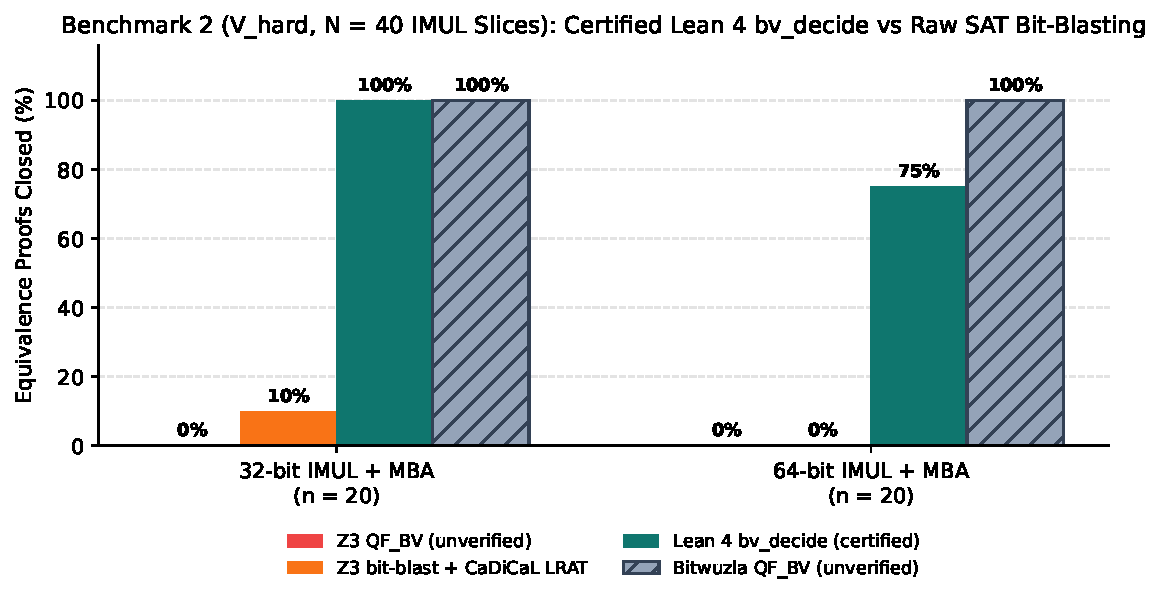
\includegraphics[width=0.78\textwidth]{fig2_vhard_lean4.pdf}
\caption{Certified proofs on $V_{\mathrm{hard}}$ (30.0\,s solver cap; strict $\le 30.0$\,s recorded time gives 2/40 = 5.0\% for CaDiCaL LRAT vs.\ 35/40 = 87.5\% for Lean 4 \texttt{bv\_decide}).}
\label{fig:vhard}
\end{figure}

\subsection{Benchmark 3: Real \texttt{gcc -O2} and \texttt{clang -O2} Compiled C Corpus ($V_{\mathrm{real}}$, $N=22$)}

Table~\ref{tab:vreal} and Figure~\ref{fig:vreal} evaluate 22 real C binaries compiled with \texttt{gcc -O2 -fno-inline} and \texttt{clang -O2 -fno-inline} from 6 candidate parameterized C templates, of which 4 templates passed the strict 17-mnemonic allowlist: 10 \texttt{affine\_mul\_64} (5 \texttt{gcc}, 5 \texttt{clang}), 10 \texttt{hash\_mix\_64} (5 \texttt{gcc}, 5 \texttt{clang}), 1 \texttt{4var\_token\_64} (\texttt{gcc}), and 1 \texttt{signed\_shift\_32} (\texttt{gcc}), while \texttt{arx\_round} and \texttt{sub\_rotate\_32} emitted instructions outside $\mathcal{M}$ under \texttt{-O2} and were excluded at freeze. Although $A$/$C$ used LRAT while $H$ used Lean~4 \texttt{bv\_decide}, in practice $A$ and $C$ failed at the search/pre-filter stage with 0 SMT passes.

\begin{table}[htbp]
\centering
\footnotesize
\resizebox{\textwidth}{!}{%
\begin{tabular}{@{}llrrrl@{}}
\toprule
\textbf{Config} & \textbf{Oracle} & \textbf{PASS / 22} & \textbf{Rate (\%)} & \textbf{Mean (s)} & \textbf{McNemar vs.\ $A \cup C$} \\
\midrule
$A$ (SiMBA + Enum) & LRAT & 0 / 22 & 0.00 & 2.28 & --- \\
$C$ (MCMC-CEGIS) & LRAT & 0 / 22 & 0.00 & 60.02* & --- \\
\texttt{H-sol} (\texttt{gpt-6.2-sol}) & Lean 4 \texttt{bv\_decide} & 6 / 22 & 27.27 & 55.12 & $p = 0.0313$ (\emph{n.s.\ at $\alpha=0.01$}) \\
\textbf{\texttt{H-hydrogen}} (\texttt{gemini-4-hydrogen}) & \textbf{Lean 4 \texttt{bv\_decide}} & \textbf{22 / 22} & \textbf{100.00} & \textbf{23.44} & \textbf{$p = 4.77 \times 10^{-7}$} \\
\bottomrule
\end{tabular}%
}
\caption{Benchmark 3 ($V_{\mathrm{real}}$, $N=22$ real \texttt{gcc/clang -O2} compiled C functions). *60.02\,s reflects 0.02\,s loop-exit overhead past the 60\,s cap.}
\label{tab:vreal}
\end{table}

\begin{figure}[htbp]
\centering
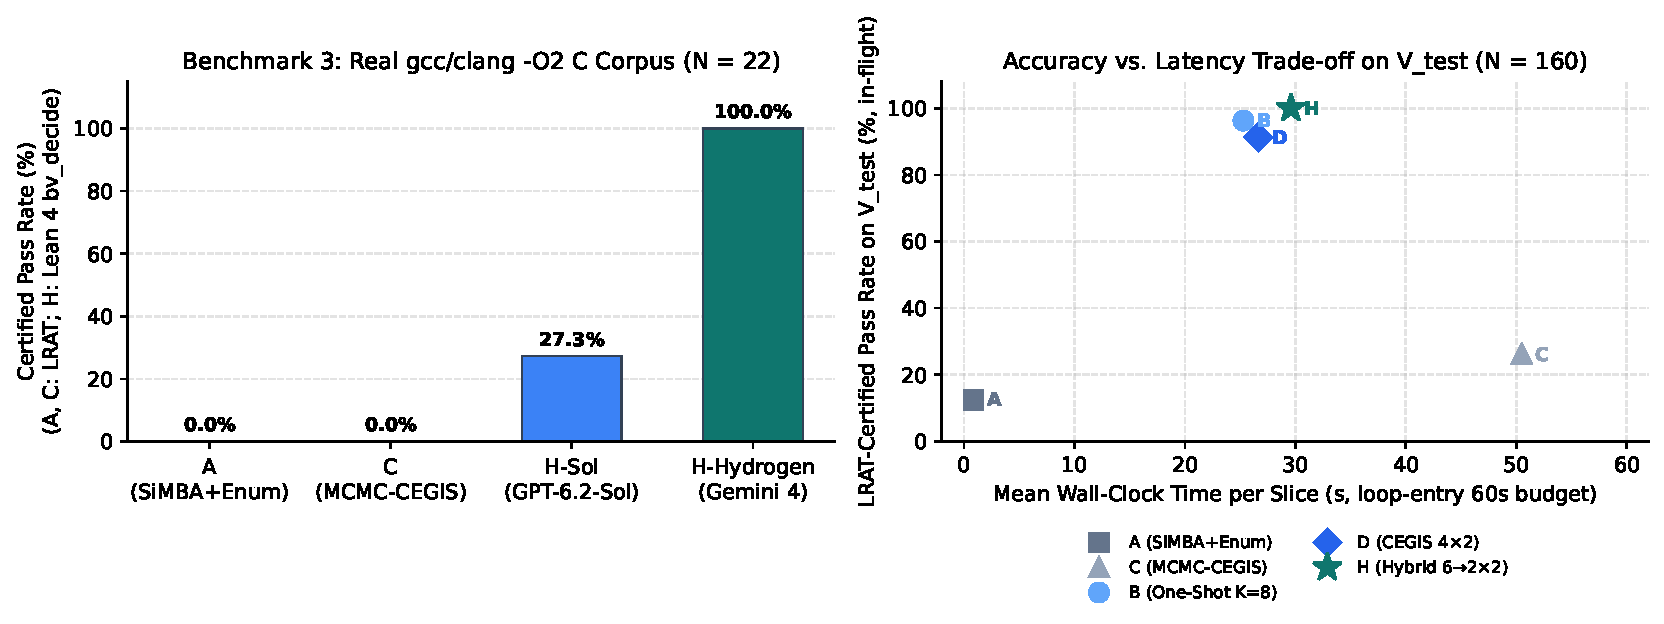
\includegraphics[width=\textwidth]{fig3_real_o2_and_tradeoff.pdf}
\caption{Left: Certified pass rates on real \texttt{gcc/clang -O2} C binaries ($V_{\mathrm{real}}$, $N=22$; $A, C$: LRAT; $H$: Lean 4 \texttt{bv\_decide}). Right: accuracy vs.\ mean wall-clock latency on $V_{\mathrm{test}}$ ($N=160$).}
\label{fig:vreal}
\end{figure}

\section{Threats to Validity, Availability, and Conclusion}

\paragraph{Threats to Validity.}
Our study intentionally restricts slices to $\le 24$ straight-line, register-only instructions without memory aliasing or unbounded loops, and discloses two freeze-stage deviations from our pre-registration document ($N=129$ vs.\ $150$ under strict $\le 10$\,s freeze LRAT certification, and byte-level rather than constant-normalized template deduplication). While Lean~4 \texttt{bv\_decide} verifies bit-blasting and checks LRAT proofs inside Lean, Lean's native evaluation axiom (\texttt{<thm>.\_native.bv\_decide.ax\_*}), \texttt{oracle\_lean.py}, and our lifter (empirically checked across 31,744 direct instruction tests plus 51,200 slice reference checks) remain in the TCB. In addition, $V_{\mathrm{real}}$ ($N=22$) is generated from 4 parameterized C templates (such as \texttt{hash\_mix\_64} and \texttt{affine\_mul\_64}) compiled with \texttt{gcc/clang -O2} whose patterns frontier LLMs may recognize from pretraining; $V_{\mathrm{real}}$ therefore evaluates certified recovery across real optimizing-compiler lowerings rather than unseen algorithm discovery. Finally, integrating external obfuscators (Tigress, OLLVM) and open-weight local models with explicit tool-free API calls is planned for v2.

\paragraph{Code and Data Availability.}
All source code, installation instructions (\texttt{README.md} + \texttt{pyproject.toml}), frozen datasets, raw benchmark JSONL/CSV logs, and an offline Artifact Evaluation script (\texttt{python3 replay\_offline.py --mode smoke} for 12 slices; \texttt{--mode full} for all 228 archived Hybrid~$H$ passes: 182 $H$-Hydrogen + 46 $H$-Sol across $V_{\mathrm{test}}$ and $V_{\mathrm{real}}$, checking cost + LRAT/Lean~4 without API keys) are archived under the MIT License at:
\begin{itemize}[leftmargin=1.5em]
  \item \textbf{Reserved Zenodo DOI (resolves upon publication):} \url{https://doi.org/10.5281/zenodo.24476603}
  \item \textbf{GitHub Repository (tag \texttt{v1.0.0}):} \url{https://github.com/larancibia/crisol-mba-x64/tree/v1.0.0}
\end{itemize}

\paragraph{Conclusion.}
Within straight-line x86-64 MBA deobfuscation, CRISOL-MBA-x64 supports $H_1$ ($+66.25$\,pp strict $\le 60$\,s on $N=160$, $p = 2.47 \times 10^{-32}$, and $+68.99$\,pp on the strict $\le 10$\,s-certified subset $N=129$, $p = 3.23 \times 10^{-27}$, with freeze deviations disclosed; while $H_2$ is not confirmed), reaches 159/160 (99.38\%, 95\% CI $[96.6\%, 100\%]$) under strict $\le 60.0$\,s and 160/160 (max 74.29\,s) in-flight with exploratory Hybrid~$H$, certifies 22/22 (95\% CI $[84.6\%, 100\%]$) \texttt{gcc/clang -O2} C binaries across 4 templates, and raises strict $\le 30.0$\,s certified \texttt{IMUL} ground-truth proofs from 5.0\% (2/40; 3/40 in-flight) to 87.5\% (35/40) via Lean~4 \texttt{bv\_decide} with 0 false positives relative to the declared TCB.

\bibliographystyle{plain}
\bibliography{references}

\end{document}
